\documentclass[11pt]{article}
\usepackage[a4paper,margin=1in]{geometry}
\usepackage{amsmath,amssymb}
\usepackage{graphicx}
\usepackage{booktabs}
\usepackage{siunitx}
\usepackage[hidelinks]{hyperref}
\usepackage{caption}

% ---- change the team name here if you want ----
\newcommand{\teamname}{Team Feynman Slaves}

\title{\vspace{-1.5em}\textbf{Physics Group Project Report}\\[0.4em]
\large An Explanatory Guide and Step-by-Step Derivation of\\
``The Pendulum --- Rich Physics from a Simple System''\\[0.3em]
\normalsize Based on the article by R. A. Nelson \& M. G. Olsson,\\
\textit{American Journal of Physics} \textbf{54}(2), 112--121 (1986)}

\author{}
\date{}

\begin{document}
\maketitle
\vspace{-3em}

\begin{center}
\begin{tabular}{ll}
\textbf{Project Group:} & \teamname{} (Group 9)\\
\textbf{Group Members:} & Bolor Ganbayar (Derivations \& mathematical layout)\\
 & Zevarniso Malakbozova (Literature review \& critical commentary)\\
 & Munkh-Iveel Vanchindorj (Computational modeling \& simulation)\\
 & Munkhtemuulen Khashbolor (Experiment, data analysis, report assembly)\\
 & \textit{All members:} experiment\\
\textbf{Course:} & General Physics I\\
\textbf{Instructor:} & Professor Deniz Olgu Devecio\u{g}lu\\
\textbf{Institution:} & Department of Physics, DGIST\\
\textbf{Date:} & June 17, 2026\\
\end{tabular}
\end{center}

\begin{abstract}
\noindent This report unpacks the foundational paper ``The Pendulum --- Rich Physics
from a Simple System'' by Nelson and Olsson. The original article shows how the
acceleration of gravity $g$ can be measured to one part in $10^4$ with a plane pendulum,
provided a long list of non-ideal corrections is applied. The published derivations
frequently compress several algebraic steps into a single line, so here we fill those
steps in explicitly, explain the physics behind each correction, and organize the
results so an introductory student can follow them. We then describe our own
small-scale reproduction of the experiment in Daegu, South Korea. Using a \SI{0.788}{m}
thread pendulum and a smartphone stopwatch, we measured $g = 10.08 \pm 0.19~\si{m/s^2}$,
about \SI{2.9}{\percent} above the accepted local value of \SI{9.797}{m/s^2}. More
importantly, we directly observed the finite-amplitude effect predicted by the paper:
the period grows with release angle, and applying the finite-amplitude correction
removes the angle dependence from our extracted value of $g$.
\end{abstract}

\tableofcontents
\bigskip

% ======================================================================
\section{Introduction and Contextual Background}

The plane pendulum is one of the oldest precision instruments in physics. Its
approximate isochronism --- first noted by Galileo --- made it the basis of accurate
mechanical clocks, and later work using pendulums provided early evidence that inertial
and gravitational mass are equivalent. For a long period the pendulum was also the most
practical laboratory method for measuring local gravity. Nelson and Olsson revisit this
``simple'' system and show that, once high accuracy is demanded, the idealized
point-mass description is no longer adequate and a surprisingly rich collection of
physical effects must be accounted for.

\subsection{Historical and Pedagogical Significance}

The central thesis of the paper is that determining $g$ to four significant figures with
an ordinary laboratory pendulum is possible, but only if one systematically computes and
applies corrections for finite swing amplitude, the finite size and mass distribution of
the bob and suspension, air buoyancy, damping, added mass, and the elasticity of the
wire and support. The intended audience is upper-level undergraduate and introductory
laboratory students: the paper is valuable precisely because it does not stop at simple
harmonic motion (as most textbooks do) but instead treats the pendulum as a real, slightly
messy object and shows how each imperfection enters the period. This is the pedagogical
move we found most useful, and it is the spirit in which we carried out our own experiment.

\subsection{Physical Setup and System Parameters}

Table~\ref{tab:symbols} lists the symbols used throughout. Where it matters we distinguish
the apparatus in the original paper (a \SI{3}{m} pendulum read with a cathetometer) from
our own apparatus (a \SI{0.79}{m} thread pendulum read with a stopwatch).

\begin{table}[h]
\centering
\caption{Key symbols, constants, and variables.}
\label{tab:symbols}
\begin{tabular}{cll}
\toprule
Symbol & Physical meaning & SI unit\\
\midrule
$m$        & Mass of the bob & \si{kg}\\
$a$        & Radius of the spherical bob & \si{m}\\
$l$ ($L_{\mathrm{eff}}$) & Effective length, pivot to centre of bob & \si{m}\\
$\theta$   & Angular displacement & \si{rad}\\
$\theta_0$ & Maximum (release) angular displacement & \si{rad}\\
$T$        & Measured period of oscillation & \si{s}\\
$T_0$      & Idealized (small-angle) period & \si{s}\\
$\omega_0$ & Natural angular frequency & \si{rad/s}\\
$I$        & Moment of inertia about the pivot & \si{kg.m^2}\\
$\rho$     & Density of air & \si{kg/m^3}\\
$g$        & Acceleration due to gravity & \si{m/s^2}\\
\bottomrule
\end{tabular}
\end{table}

% ======================================================================
\section{Step-by-Step Mathematical Derivations}

\subsection{The Starting Framework}

A point mass on a massless, inextensible cord of length $l$ swinging in a vacuum obeys
the torque equation
\begin{equation}
\ddot{\theta} + \frac{g}{l}\sin\theta = 0 .
\label{eq:eom}
\end{equation}
For infinitesimal displacements we expand $\sin\theta \approx \theta$, and
Eq.~\eqref{eq:eom} reduces to the simple-harmonic form $\ddot{\theta}+\omega_0^2\theta=0$
with $\omega_0^2 = g/l$. The solution oscillates at the natural frequency $\omega_0$, so
the idealized period is
\begin{equation}
T_0 = 2\pi\sqrt{\frac{l}{g}} = \frac{2\pi}{\omega_0}.
\label{eq:T0}
\end{equation}
Rearranging Eq.~\eqref{eq:T0} gives the working equation that converts a measured length
and period into gravity:
\begin{equation}
g = \frac{4\pi^2 l}{T_0^{2}}.
\label{eq:g}
\end{equation}

\subsection{Filling in the Missing Step: the Correction Framework}

A real pendulum never has the ideal period. The paper writes the measured period as the
ideal period plus a cumulative offset,
\begin{equation}
T = T_0 + \Delta T = T_0\!\left(1 + \frac{\Delta T}{T_0}\right).
\label{eq:framework}
\end{equation}
To recover the ideal $T_0$ from the measured $T$ we divide and expand. Because every
individual correction is tiny ($\Delta T/T_0 \ll 1$), a first-order binomial expansion
$(1+x)^{-1}\approx 1-x$ is justified:
\begin{equation}
T_0 = \frac{T}{1 + \Delta T/T_0} \approx T\!\left(1 - \frac{\Delta T}{T_0}\right).
\label{eq:T0recover}
\end{equation}
The strategy of the paper is therefore: measure $T$, compute every contribution to
$\Delta T/T_0$ separately, add them (they are small enough to add linearly), and feed the
corrected $T_0$ into Eq.~\eqref{eq:g}.

% ======================================================================
\section{Physical Corrections and Limiting Cases}

This section reconstructs the dominant corrections of the paper, evaluated for the
\emph{original} apparatus ($a=\SI{3.05}{cm}$, $l=\SI{300.44}{cm}$, $\theta_0=\ang{3.0}$).
We later show in Section~\ref{sec:experiment} that, at our much coarser precision, only
the first of these is large enough to matter.

\subsection{Finite-Amplitude Correction}
The linear approximation $\sin\theta\approx\theta$ breaks down for finite swings. An exact
treatment of Eq.~\eqref{eq:eom} via energy conservation gives the period as a complete
elliptic integral of the first kind, $K(k)$, with $k=\sin(\theta_0/2)$:
\begin{equation}
T = \frac{4}{\omega_0}\,K\!\left(\sin\tfrac{\theta_0}{2}\right).
\end{equation}
Expanding $K$ as a power series and integrating term by term yields
\begin{equation}
\frac{\Delta T}{T_0} = \frac{1}{16}\,\theta_0^{2} + \frac{11}{3072}\,\theta_0^{4} + \cdots
\label{eq:famp}
\end{equation}
For $\theta_0=\ang{3.0}$ the leading term gives $\Delta T \approx +\SI{596}{\micro s}$:
larger swings genuinely take longer. This is the single most important correction and the
one we were able to observe directly in our own data.

\subsection{Mass-Distribution Corrections}
A real bob has finite size, so the system is a \emph{physical} pendulum with period
\begin{equation}
T = 2\pi\sqrt{\frac{I}{Mgh}},
\label{eq:physpend}
\end{equation}
where $I$ is the moment of inertia about the pivot, $M$ the total mass, and $h$ the
pivot-to-centre-of-mass distance. For a uniform sphere of radius $a$ on a massless cord,
the parallel-axis theorem gives $I = ml^2\!\left[1+\tfrac{2}{5}(a/l)^2\right]$ with $M=m$,
$h=l$, so
\begin{equation}
\frac{\Delta T}{T_0} = \frac{1}{5}\left(\frac{a}{l}\right)^{2}.
\label{eq:radius}
\end{equation}
For the paper's apparatus this is $+\SI{72}{\micro s}$. The suspension ring, attachment
cap, cap screw, and the distributed mass of the wire each add further small terms; the
wire mass alone shortens the period by $\Delta T/T_0 = -\tfrac{1}{12}(m_w/m)$, about
$-\SI{463}{\micro s}$ in the original experiment.

\subsection{Air Corrections}
The surrounding air contributes in three ways. \emph{Buoyancy} reduces the bob's apparent
weight (Archimedes), which weakens the effective restoring ``gravity'' and lengthens the
period:
\begin{equation}
\frac{\Delta T}{T_0} = \frac{1}{2}\,\frac{m_a}{m},
\label{eq:buoyancy}
\end{equation}
giving $+\SI{292}{\micro s}$ for the paper. \emph{Damping} (a combination of linear and
quadratic air drag) slightly increases the period, and \emph{added mass} --- the air
dragged along with the bob --- increases the system's effective inertia, contributing
about $+\SI{346}{\micro s}$.

\subsection{Elastic Corrections}
Finally, neither the wire nor the support is perfectly rigid. Static and dynamic stretching
of the wire and small lateral motion of the mounting point each shift the period, but for
the paper's stiff steel wire and massive support these terms are at the microsecond level
or below.

\subsection{Summary of the Paper's Corrections}
Table~\ref{tab:corrections} collects the corrections for the original apparatus. Their
sum, $\Delta T = +\SI{472}{\micro s}$, converts the naive measurement into
$T_0 = \SI{3.47833}{s}$ and hence $g = \SI{9.8034 \pm 0.0014}{m/s^2}$, in agreement with
the independently known local value --- the headline success of the paper.

\begin{table}[h]
\centering
\caption{Dominant corrections for the original Nelson--Olsson apparatus.}
\label{tab:corrections}
\begin{tabular}{lr}
\toprule
Effect & $\Delta T$ ($\si{\micro s}$)\\
\midrule
Finite amplitude        & $+596$\\
Finite radius of bob    & $+72$\\
Mass of ring            & $-282$\\
Mass of cap             & $-116$\\
Mass of cap screw       & $+95$\\
Mass of wire            & $-463$\\
Buoyancy                & $+292$\\
Added mass              & $+346$\\
Damping (net)           & $\sim -44$\\
Elastic / support       & $\sim +4$\\
\midrule
\textbf{Total}          & $\mathbf{+472}$\\
\bottomrule
\end{tabular}
\end{table}

% ======================================================================
\section{Experimental Reproduction and Results}
\label{sec:experiment}

To put the paper's framework into practice we built and timed a simple pendulum and
extracted $g$ from our own data.

\subsection{Apparatus and Setup}
The bob was a steel ball of mass $m = \SI{200.0 \pm 0.1}{g}$ and radius
$a = \SI{1.35}{cm}$, suspended on a thin thread. The effective length, measured from the
pivot to the centre of the ball after the setup was finalized, was
$L_{\mathrm{eff}} = \SI{78.8}{cm}$. The experiment was carried out in Daegu, South Korea,
where the accepted local gravity is \SI{9.797}{m/s^2}.

\subsection{Engineering Iterations}
Our raw setup did not behave ideally, and dealing with this is itself an illustration of
the paper's theme that a real pendulum departs from the ideal. Three problems and fixes
are worth recording. (i)~A loosely tied knot let the bob pivot about a second point, so
the system briefly behaved as a \emph{double pendulum}; inserting a small wood piece at
the knot fixed the pivot and stopped this motion. (ii)~The thread swung slightly forward
and back rather than in a single plane; closing the gap between the support and the thread
constrained it. (iii)~Releasing the bob by hand introduced sideways motion, so we released
it against a foam board for a consistent, push-free start. Each fix made the timing more
repeatable, and --- importantly --- the knot/support changes are what set the final
effective length.

\subsection{Procedure and Timing Data}
For each release angle we timed $N=20$ complete oscillations and repeated for six trials.
We used angles of \ang{5}, \ang{10}, \ang{15}, and \ang{20}, with a single \ang{30} trial.
Table~\ref{tab:timing} reports the mean time, sample standard deviation, the mean period
$\bar{T}=\bar{t}/20$, the finite-amplitude factor from Eq.~\eqref{eq:famp}, and the
corrected small-angle period $T_0 = \bar{T}/(1+\theta_0^2/16+11\theta_0^4/3072)$.

\begin{table}[h]
\centering
\caption{Timing data and finite-amplitude correction ($N=20$ oscillations).}
\label{tab:timing}
\begin{tabular}{cccccc}
\toprule
$\theta_0$ & $\bar{t}_{20}$ (s) & $s$ (s) & $\bar{T}$ (s) & amplitude factor & $T_0$ (s)\\
\midrule
\ang{5}  & 35.150 & 0.079 & 1.7575 & 1.000476 & 1.7567\\
\ang{10} & 35.128 & 0.069 & 1.7564 & 1.001907 & 1.7531\\
\ang{15} & 35.343 & 0.137 & 1.7672 & 1.004301 & 1.7596\\
\ang{20} & 35.435 & 0.044 & 1.7718 & 1.007669 & 1.7583\\
\ang{30} & 36.770 & --- & 1.8385 & 1.017404 & 1.8071\\
\bottomrule
\end{tabular}
\end{table}

The \ang{30} point has only one trial, so we exclude it from the final analysis and use it
only as a qualitative consistency check.

\subsection{Extracting $g$}
Applying $g = 4\pi^2 L_{\mathrm{eff}}/T^2$ to both the \emph{raw} mean period and the
\emph{corrected} period gives Table~\ref{tab:gvals}. The contrast between the two columns
is the key result, shown in Fig.~\ref{fig:gangle}.

\begin{table}[h]
\centering
\caption{Gravity extracted from the raw and corrected periods.}
\label{tab:gvals}
\begin{tabular}{ccc}
\toprule
$\theta_0$ & $g_{\mathrm{raw}}$ (\si{m/s^2}) & $g_{\mathrm{corrected}}$ (\si{m/s^2})\\
\midrule
\ang{5}  & 10.072 & 10.081\\
\ang{10} & 10.084 & 10.123\\
\ang{15} & 9.962  & 10.048\\
\ang{20} & 9.910  & 10.063\\
\midrule
mean     & 10.007 & 10.079\\
spread (SD) & 0.085 & 0.032\\
\bottomrule
\end{tabular}
\end{table}

\begin{figure}[h]
\centering
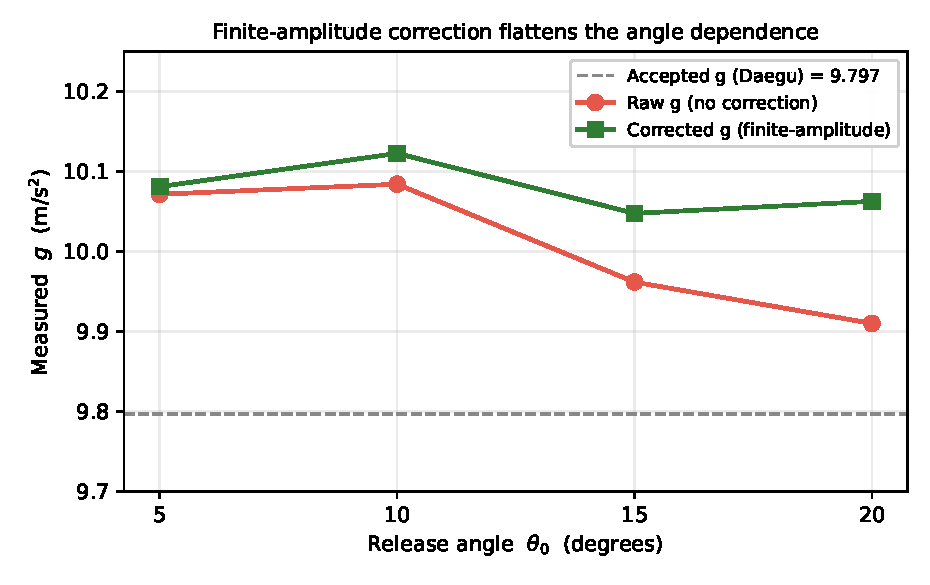
\includegraphics[width=0.78\textwidth]{g_vs_angle.pdf}
\caption{Gravity extracted at each release angle. The raw values (red) fall as the angle
increases, because larger swings have longer periods. Applying the finite-amplitude
correction (green) removes this trend and leaves a nearly flat value of $g$. Both lie
about \SI{3}{\percent} above the accepted local value (dashed), reflecting the dominant
uncertainty in the effective length.}
\label{fig:gangle}
\end{figure}

\subsection{Final Value and Error Analysis}
Averaging the four corrected angles gives
\begin{equation}
g = 10.08 \pm 0.19~\si{m/s^2},
\end{equation}
about $+\SI{2.87}{\percent}$ relative to the accepted \SI{9.797}{m/s^2}, which lies roughly
$1.5$ standard deviations below our mean. The uncertainty is dominated by the effective
length: propagating
\begin{equation}
\left(\frac{\sigma_g}{g}\right)^2 = \left(\frac{\sigma_L}{L_{\mathrm{eff}}}\right)^2 +
\left(\frac{2\sigma_T}{T_0}\right)^2,
\label{eq:errprop}
\end{equation}
the timing term is negligible (our corrected $g$ values agree across angles to $\pm0.03$),
whereas a realistic length uncertainty of $\sigma_L \approx \SI{1.5}{cm}$ --- arising from
the difficulty of locating the true pivot after the knot and support were adjusted ---
accounts for essentially the entire error bar.

\subsection{Which Corrections Matter at Our Scale}
A useful exercise is to ask which of the paper's corrections are even relevant for our
crude apparatus. The finite-amplitude term is large: between \ang{5} and \ang{20} it
shifts the period by about \SI{0.7}{\percent}, which is exactly the trend removed in
Fig.~\ref{fig:gangle}. By contrast, the finite-bob-radius term of Eq.~\eqref{eq:radius}
evaluates to $\tfrac{1}{5}(1.35/78.8)^2 \approx 6\times10^{-5}$, i.e. a
\SI{0.006}{\percent} effect on the period, and the wire-mass and buoyancy terms are
similarly small. We therefore applied only the finite-amplitude correction and neglected
the rest --- a deliberate choice that reflects the precision of a stopwatch-and-thread
experiment, rather than an oversight.

% ======================================================================
\section{Critical Analysis and Commentary}

The idealized formulae rest on several assumptions: negligible air resistance and buoyancy,
a perfectly rigid and inextensible suspension, a point-mass bob, and a fixed pivot. The
paper's real contribution is to show that these assumptions are not merely approximations
to be waved away but each correspond to a measurable, calculable shift in the period. At
small angles and modest precision the assumptions hold well, but as accuracy demands grow,
the non-ideal effects become significant and the analysis must become correspondingly more
realistic.

A second implicit assumption is that the measurements themselves are exact. In practice the
length, period, mass, and damping all carry uncertainty, and our own experiment makes the
consequences concrete: our result is limited not by timing but by how well we could define
the effective length. The paper is somewhat light on this practical side --- it focuses on
the theory of the corrections rather than on the day-to-day difficulty of building a clean
pendulum --- and our experience suggests that connecting the elegant corrections to the
messiness of real data collection deserves more emphasis.

The strength of the paper is pedagogical: it demonstrates how a deceptively simple system
can display rich behaviour once examined carefully, and how a basic model can be refined
step by step into a precision instrument. The same logic extends well beyond pendulums ---
to seismometers, mechanical clocks, earthquake engineering, and any oscillatory system
where damping and nonlinearity matter.

% ======================================================================
\section{Conclusion}

We reconstructed the central derivations of Nelson and Olsson, supplying the intermediate
algebra the paper compresses, and explained the physical origin of each correction to the
ideal pendulum period. We then reproduced the experiment at introductory scale. Our
measured value, $g = 10.08 \pm 0.19~\si{m/s^2}$, is about \SI{2.9}{\percent} high, with the
discrepancy traceable to the uncertainty in the effective length rather than to the timing.
Most satisfying, our multi-angle data reproduced the paper's central qualitative claim: the
period lengthens with amplitude, and the finite-amplitude correction --- the only one large
enough to matter at our precision --- flattens the angle dependence in the extracted $g$.
Working through both the theory and a hands-on measurement made clear why even a ``simple''
pendulum repays careful analysis, and how unpacking each approximation connects the
mathematics to the behaviour of a real physical system.

% ======================================================================
\section*{Code and Data Availability}
The interactive simulation, raw timing data, this report, and its \LaTeX{} source are
available at:
\begin{center}
\url{https://github.com/Iveel17/physics_project}
\end{center}
A live interactive demonstration is hosted at
\url{https://iveel17.github.io/physics_project/}.

% ======================================================================
\begin{thebibliography}{9}
\bibitem{nelson} R. A. Nelson and M. G. Olsson, ``The pendulum --- Rich physics from a
simple system,'' \textit{American Journal of Physics} \textbf{54}(2), 112--121 (1986).
\bibitem{prelab} Course laboratory handout, ``Measurement of Gravitational Acceleration
Using a Simple Pendulum,'' General Physics I, DGIST (2026).
\bibitem{marion} J. B. Marion and S. T. Thornton, \textit{Classical Dynamics of Particles
and Systems}, 5th ed. (Brooks/Cole, 2003).
\end{thebibliography}

\end{document}
